\documentclass[tikz,border=5mm]{standalone}
\usetikzlibrary{shapes.geometric, arrows.meta, positioning, fit, backgrounds}
\begin{document}
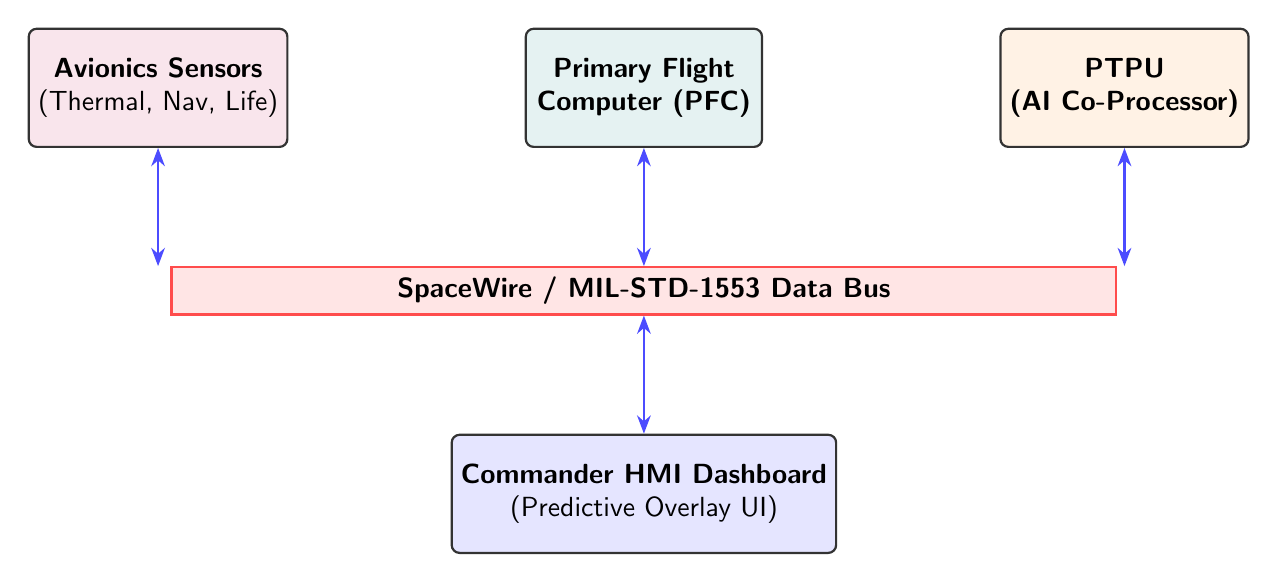
\begin{tikzpicture}[
    font=\sffamily,
    box/.style={rectangle, draw=black!80, fill=white, thick, rounded corners=1mm, minimum width=3cm, minimum height=1.5cm, align=center},
    bus/.style={rectangle, draw=red!70, fill=red!10, thick, minimum width=12cm, minimum height=0.6cm, align=center},
    arrow/.style={<->, >=Stealth, thick, draw=blue!70}
]

\node[bus] (bus) {\textbf{SpaceWire / MIL-STD-1553 Data Bus}};

\node[box, fill=purple!10, above left=1.5cm and -1.5cm of bus] (sensors) {\textbf{Avionics Sensors}\\(Thermal, Nav, Life)};
\node[box, fill=teal!10, above=1.5cm of bus] (pfc) {\textbf{Primary Flight}\\\textbf{Computer (PFC)}};
\node[box, fill=orange!10, above right=1.5cm and -1.5cm of bus] (ptpu) {\textbf{PTPU}\\\textbf{(AI Co-Processor)}};

\node[box, fill=blue!10, below=1.5cm of bus] (hmi) {\textbf{Commander HMI Dashboard}\\(Predictive Overlay UI)};

\draw[arrow] (sensors.south) -- (sensors.south |- bus.north);
\draw[arrow] (pfc.south) -- (pfc.south |- bus.north);
\draw[arrow] (ptpu.south) -- (ptpu.south |- bus.north);
\draw[arrow] (hmi.north) -- (hmi.north |- bus.south);

\end{tikzpicture}
\end{document}
